% One-shot decorator.
\documentclass[border=6pt,tikz]{standalone}
\usepackage{tikz}
\usepackage{amsmath, amssymb}
\usepackage[T1]{fontenc}
\usepackage{lmodern}
\usetikzlibrary{arrows.meta, positioning}

\tikzset{
  decorator/.style = {draw, rounded corners=2pt, fill=purple!12, align=center,
                      font=\small, inner sep=4pt, minimum width=2.2cm, minimum height=0.9cm},
  child/.style     = {draw, rounded corners=2pt, fill=yellow!18, align=center,
                      font=\scriptsize, inner sep=3pt, minimum width=1.6cm, minimum height=0.7cm},
  flow/.style      = {-, line width=0.55pt},
}

\begin{document}
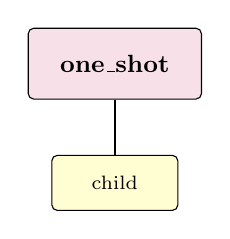
\begin{tikzpicture}[node distance=0.7cm]
  \node[decorator]              (d) {\textbf{one\_shot}};
  \node[child, below=of d]      (c) {child};
  \draw[flow] (d) -- (c);
\end{tikzpicture}
\end{document}
